\section{PRELIMINARIES}
\label{sect:preliminaries}
%Describe the concepts of the paper topic. Then, setup a formal definition for the research problem we address in this paper. state the assumptions, and definitions as needed to frame the boundaries of this work.

\subsection{Background}
% Establish the needed basics for the project
%Spatial Data processing
Spatial data is as known as geospatial data or geographic information it is the data or information that identifies the geographic location of features and boundaries on Earth, such as natural or constructed features, oceans, and more. Spatial data is usually stored as coordinates and topology, and is data that can be mapped. Generally speaking, spatial data represents the location, size and shape of an object on planet Earth such as a building, lake, mountain or township. Spatial data may also include attributes that provide more information about the entity that is being represented. Geographic Information Systems (GIS) or other specialized software applications can be used to access, visualize, manipulate and analyze geospatial data.


Support of high performance queries on large volumes of spatial
data becomes increasingly important in many application domains,
including geospatial problems in numerous fields, location based
services, and emerging scientific applications that are increasingly
data-intensive and compute-intensive. There are two major challenges for managing and querying
massive spatial data to support spatial queries: the explosion of spatial data, and the high computational complexity of spatial queries.

% Hadoop
Apache Hadoop is an open-source software framework for distributed storage and distributed processing of very large data sets on computer clusters built from commodity hardware. All the modules in Hadoop are designed with a fundamental assumption that hardware failures are common and should be automatically handled by the framework.

The core of Apache Hadoop consists of a storage part, known as Hadoop Distributed File System (HDFS), and a processing part called MapReduce. Hadoop splits files into large blocks and distributes them across nodes in a cluster. To process data, Hadoop transfers packaged code for nodes to process in parallel based on the data that needs to be processed. This approach takes advantage of data locality to allow the dataset to be processed faster and more efficiently than it would be in a more conventional supercomputer architecture that relies on a parallel file system where computation and data are distributed via high-speed networking. 

The base Apache Hadoop framework is composed of the following modules: (i) Hadoop Common contains libraries and utilities needed by other Hadoop modules; (ii) Hadoop Distributed File System (HDFS) is a distributed file-system that stores data on commodity machines, providing very high aggregate bandwidth across the cluster; (iii)Hadoop YARN is a resource-management platform responsible for managing computing resources in clusters and using them for scheduling of users' applications; and (iv)Hadoop MapReduce is an implementation of the MapReduce programming model for large scale data processing.

% SpatialHadoop
SpatialHadoop \cite{eldawy2015spatialhadoop}, a MapReduce Framework for Spatial Data, is designed and implemented by Dr.Eldawy in 2015. SpatialHadoop is an open source MapReduce extension designed specifically to handle huge datasets of spatial data on Apache Hadoop. It is shipped with built-in spatial high level language, spatial data types, spatial indexes and efficient spatial operations. It provides spatial data types to be used in MapReduce jobs including point, rectangle and polygon. It also adds low level spatial indexes in HDFS such as Grid file, R-tree and R+-tree. Some new InputFormats and RecordReaders are also provided to allow reading and processing spatial indexes efficiently in MapReduce jobs. SpatialHadoop also ships with a bunch of spatial operations that are implemented as efficient MapReduce jobs which access spatial indexes using the new components. Developers can implement myriad spatial operations that run efficiently using spatial indexes.


\subsection{Problem Definition}
% Formalize the problem in terms of inputs, outputs, query/research-question, and objectives, e.g., reduce/min/max (accuracy, efficiency, distance, idle-time, etc)

%input output and query speed 
SpatialHadoop can handle large amount of spatial dataset processing since it leverages the distributed big data computation framework Hadoop and MapReduce \cite{dean2008mapreduce} model. Based on users' own needs, they can specify and develop the corresponding operations such as range query, k-nearest neighbor and spatial join. After the query operation in SpatialHadoop system, a result report will be generated under the HDFS. However, when spatial data scales to large dataset, this spatial data operations is still time consuming. To improve the query speed performance of spatial data processing, the under-layer functionalities can still be optimized. 

% objective :
The object of this work is to extend the MapReduce layer of SpatialHadoop framework for improving the time efficiency of spatial data processing.


\subsection{Solution Architecture}
\label{subsec:architecture}

The architecture of the SpatialHadoop system is given in Figure~\ref{fig:architecture}.
\begin{figure}[htb!]
\centering
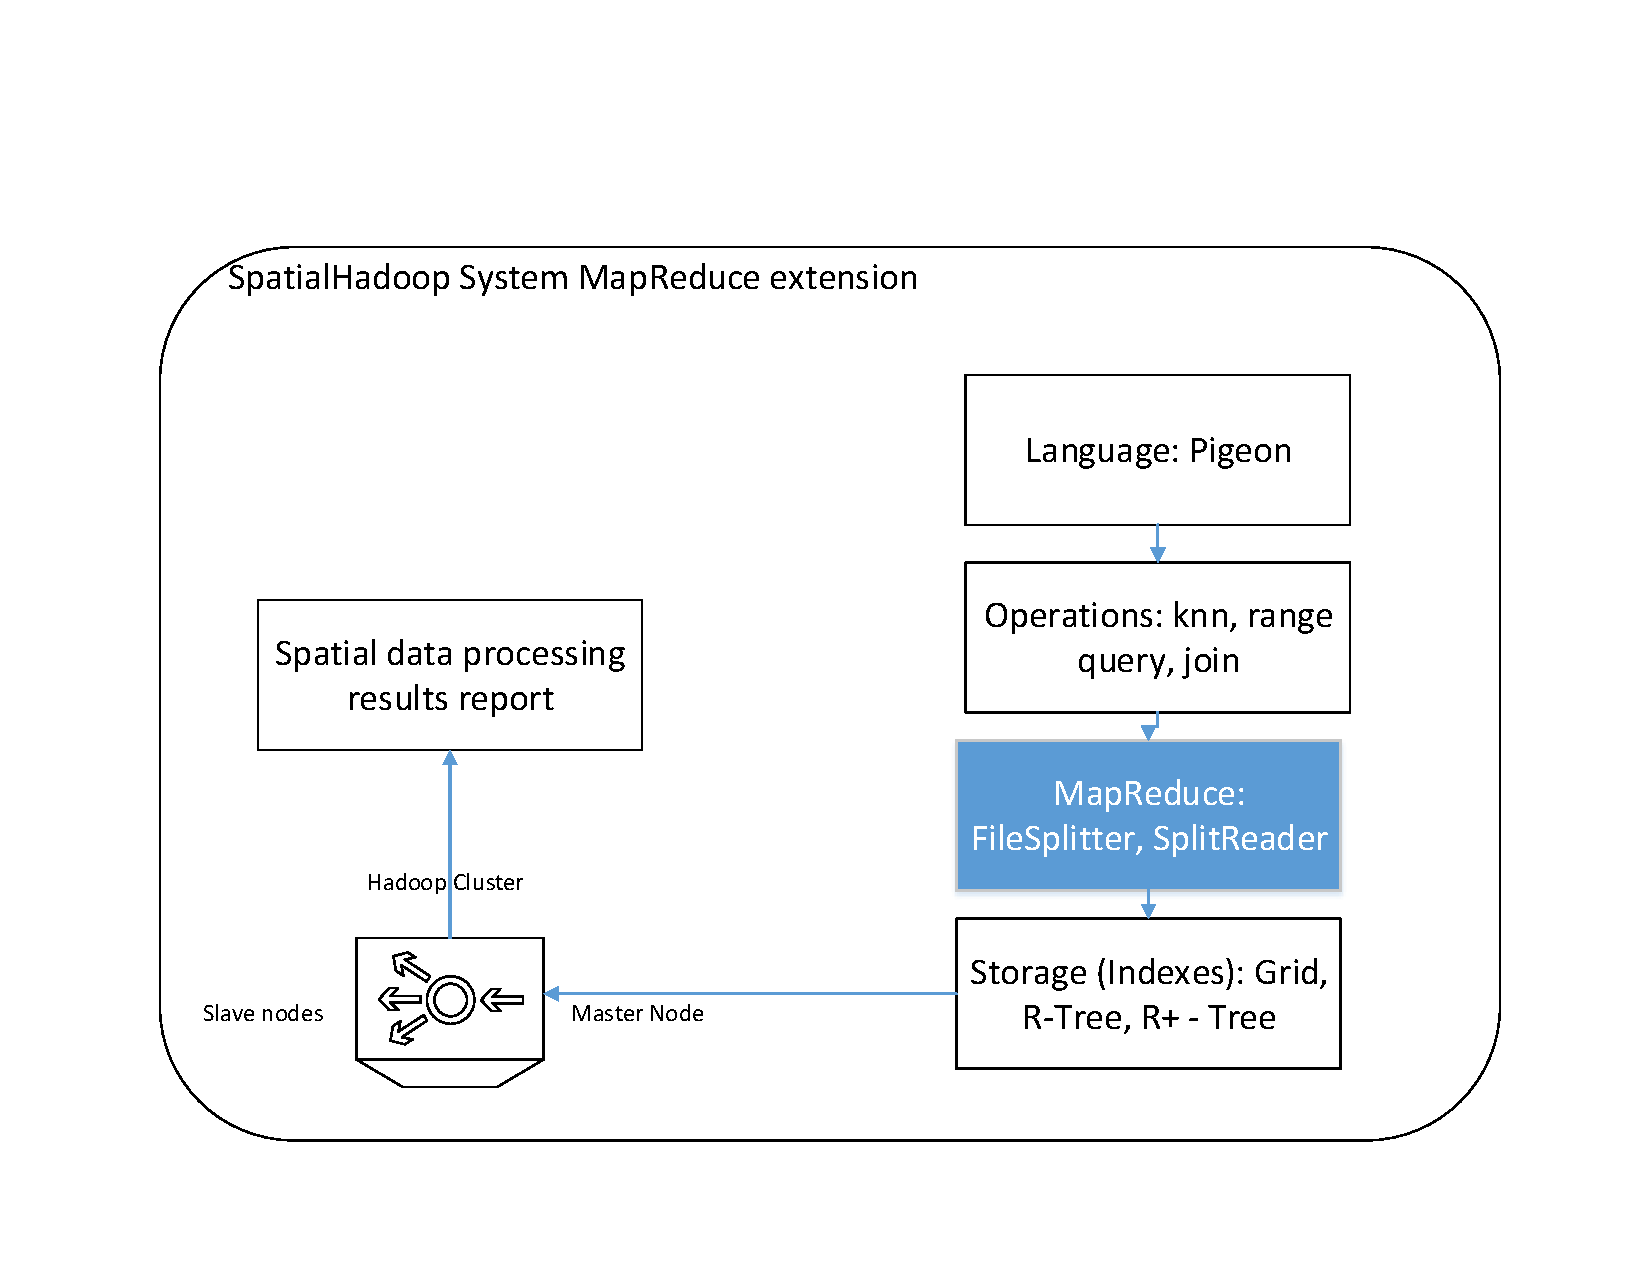
\includegraphics[width=0.90\columnwidth]{figures/architecture.pdf}
\caption{SpatialHadoop system with extension architecture}
\label{fig:architecture}
\end{figure}

% Describe briefly the main modules of the system and the employed data structures.
% We say briefly here as we will dedicate a separate section for each main module or part in the system.

As Fig.~\ref{fig:architecture} presents, SpatialHadoop cluster use the similar computation model as Hadoop. The cluster consists of a master node that breaks a MapReduce job into smaller tasks, then a bunch of slave nodes process the smaller tasks individually. Based on the original SpatialHadoop design \cite{eldawy2015spatialhadoop}, there are mainly two type of users can use this system. (i) Casual users who do not know much about the computing and programming can access this system through a spatial language to process their datasets. (ii) Developer or data scientists who have a deeper understanding of the system and can implement their new spatial operation based on what they need, or they can just simply use the SpatialHadoop command line started with \texttt{shadoop}. Basically, it is a compile binary executable file give users access to the spatial operations by commands. 

The language layer provides a simple high level SQL-like language Pigeon \cite{eldawy2014pigeon}, which is complant spatial data types like point and Polygon, and spatial operations like overlap and touches for simplifying spatial data processing. 

The operations layer encapsulates the implementation of various spatial operations that take advantage of spatial indexes and the new components in the MapReduce layer. The most common three spatial data operations provided are range query, kNN, and spatial join. In this paper, the performance measurements were mainly evaluated through the kNN query.

The MapReduce mainly has two components to allow MapReduce program to access the spatial index structures. The SpatialFileSplitter exploits the global index to prune file blocks that is not the possible query results, and SpatialRecorderReader exploits local indexex to efficiently retrieve a partial answer from each block. We improved the SpatialFileSplitter with a new class called \texttt{FileSplitUtil} which provides a more flexible way to split the big spatial data file block and combine them based on knn query accuracy (With different k values).

Since inputs files in Hadoop are non-indexed heap files, the performance is limited as the input scales. The SpatialHadoop employs spatial index structures within Hadoop Distributed File System (HDFS) as a means of efficient retrieval of spatial data. Indexing in SpatialHadoop is the main reason in its better time efficiency over normal Hadoop. To overcome the challenges of building index structures in Hadoop, the SpatialHadoop system uses a two-layers indexing approach of global and local index as shown in Fig.~\ref{fig:index}. Each index contains one global index stored in the Master node, that partitions data across a set of partitions, stored in slaves nodes. This indexing organization lends itself to MapReduce programming, where the local indexes can be processed in a MapReduce job. And the small size of local indexes allows each one to be bulk loaded in memory and written to a file in an append-only manner. Also, indexing in SpatialHadoop adapts HDFS to accommodate general purpose standard spatial index structures, namely, Grid file, R-tree, R+-Tree, and use them to support to support many spatial many spatial queries written in MapReduce. In this paper, we mainly use the Grid as the default indexing method for evaluation purpose.

\begin{figure}[htb!]
\centering
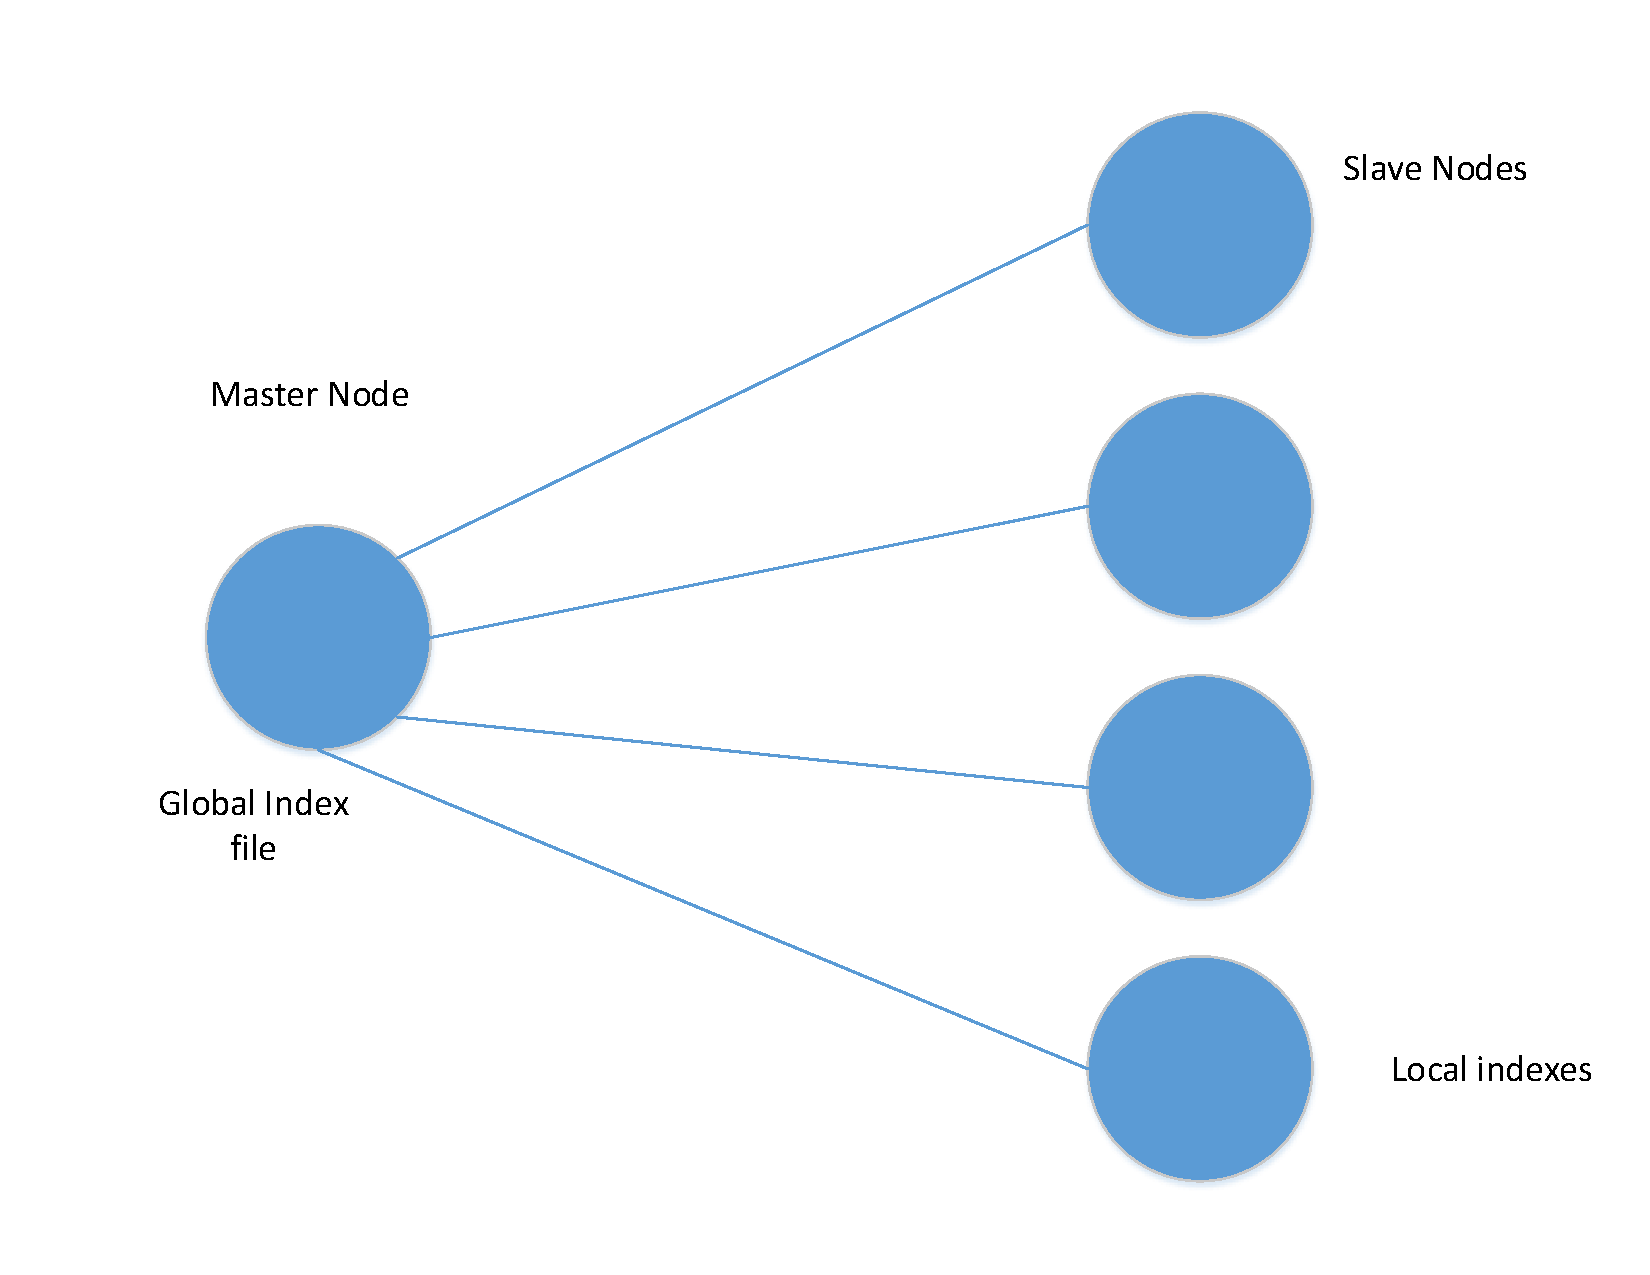
\includegraphics[width=0.90\columnwidth]{figures/Index.pdf}
\caption{SpatialHadoop two layer indexing}
\label{fig:index}
\end{figure}





%%$$$$$$$$$$$$$$$$$$$$$$$$$$$$$$$$$$$$$$$$$$$$$$$$$$$$$$$$$$$$$$$$$$$
%\begin{figure}[t]
%  \begin{center}
%  %width=2.818in
%  \includegraphics[width=0.90\columnwidth]{SystemArchitecture.eps}
%  \vspace{-10pt}
%  \caption{The Architecture Of The {\em W} System}
%  \label{fig:architecture}
%  \vspace{-20pt}
%  \end{center}
%\end{figure}
%%$$$$$$$$$$$$$$$$$$$$$$$$$$$$$$$$$$$$$$$$$$$$$$$$$$$$$$$$$$$$$$$$ 


\subsection{Data Structures}
\label{subsec:dataStructures}
% Provide detailed explanation about the employed or the introduced data structures here. 
In terms of data structure used in this paper, three indexing data structure are introduced as the previous section. While the main three phases of indexing, which is partitioning, local indexing, and global indexing, several steps are done by the indexing system. Certain algorithm are used to decide the number of partitions and the partitions boundaries. For the purpose of building requested local index on the data contents of each physical partition. This is implemented as a \texttt{reduce} function that takes the small records and stores the in a spatial index written in a local index file. Each local index fits in one HDFS block about 64 MB. Mainly, two type of data structure are used. The first is Grid indexing structure, the second is R tree. 

Grid indexing is a regular tessellation of a manifold or 2-D surface that divides it into a series of contiguous cells, which can then be assigned unique identifiers and used for spatial indexing purposes. A wide variety of such grids have been proposed or are currently in use, including grids based on "square" or "rectangular" cells, triangular grids or meshes, hexagonal grids and grids based on diamond-shaped cells. In practice, construction of grid-based spatial indices entails allocation of relevant objects to their position or positions in the grid, then creating an index of object identifiers vs. grid cell identifiers for rapid access. This is an example of a "space-driven" or data independent method, as opposed to "data-driven" or data dependent method. A grid-based spatial index has the advantage that the structure of the index can be created first, and data added on an ongoing basis without requiring any change to the index structure; indeed, if a common grid is used by disparate data collecting and indexing activities, such indices can easily be merged from a variety of sources. On the other hand, data driven structures such as R-trees can be more efficient for data storage and speed at search execution time, though they are generally tied to the internal structure of a given data storage system. Fig.~\ref{fig:grid} shows how to use grid indexing to partition the spatial data and build the indexes.
 
\begin{figure}[htb!]
\centering
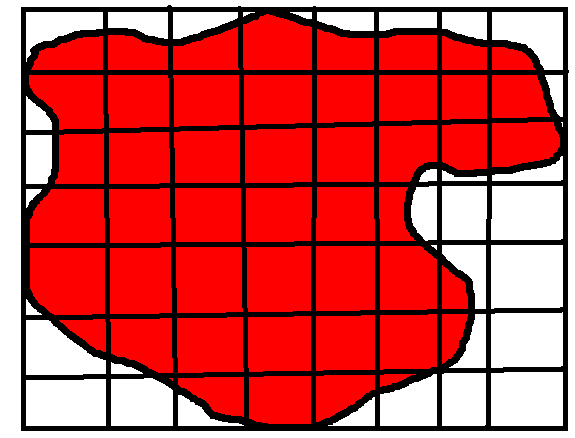
\includegraphics[width=0.90\columnwidth]{figures/grid.png}
\caption{Grid indexing partitioning}
\label{fig:grid}
\end{figure}
 
 R-trees are tree data structures used for spatial access methods, i.e., for indexing multi-dimensional information such as geographical coordinates, rectangles or polygons. A common real-world usage for an R-tree might be to store spatial objects such as restaurant locations or the polygons that typical maps are made of: streets, buildings, outlines of lakes, coastlines, etc. The R-tree can also accelerate nearest neighbour search for various distance metrics, including great-circle distance. Fig.~\ref{fig:rtree}
 
 \begin{figure}[htb!]
\centering
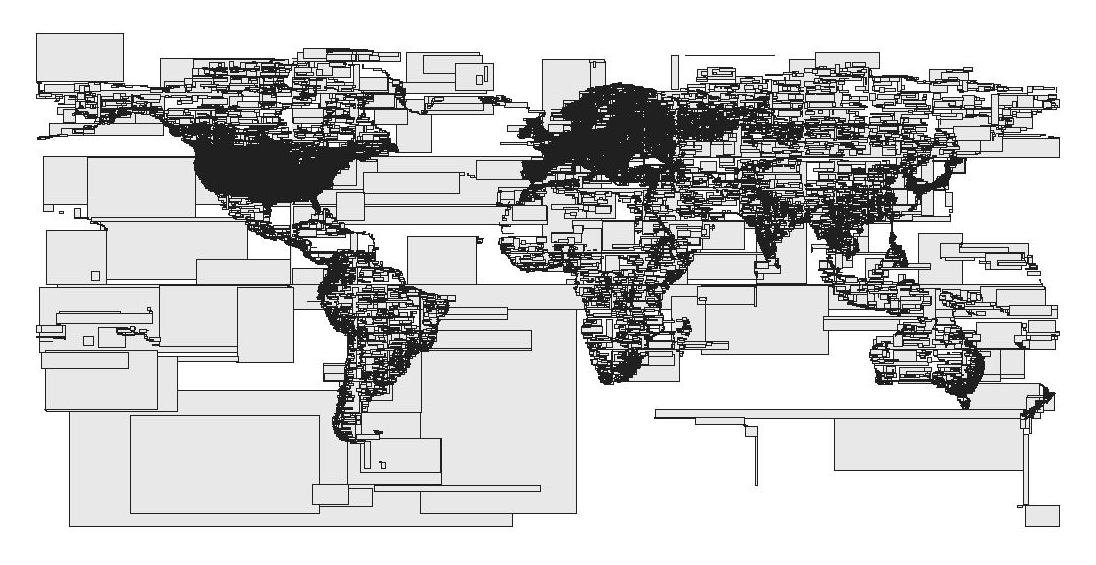
\includegraphics[width=0.90\columnwidth]{figures/Rtree.png}
\caption{Rtree indexing partitioning}
\label{fig:rtree}
\end{figure}

The key idea of the data structure is to group nearby objects and represent them with their minimum bounding rectangle in the next higher level of the tree; the ``R'' in R-tree is for rectangle. Since all objects lie within this bounding rectangle, a query that does not intersect the bounding rectangle also cannot intersect any of the contained objects. At the leaf level, each rectangle describes a single object; at higher levels the aggregation of an increasing number of objects. This can also be seen as an increasingly coarse approximation of the data set.
